\documentclass{letask}
\usepackage{gnuplottex}
\usepackage{epstopdf}
\usepackage{cancel}
\usepackage{icomma}
\begin{document}
\begin{titlepage}
\center % Center everything on the page
 
%----------------------------------------------------------------------------------------
%	HEADING SECTIONS
%----------------------------------------------------------------------------------------

\textsc{\LARGE Московский\\[-0.2cm]Физико-Технический Институт\\[0.1cm]\large (государственный университет)}\\[1.5cm] % Name of your university/college
\textsc{\Large Кафедра общей физики}\\[0.1cm] % Major heading such as course name
\textsc{\large Вопрос по выбору, 3 семестр}\\[0.5cm] % Minor heading such as course title

%----------------------------------------------------------------------------------------
%	TITLE SECTION
%----------------------------------------------------------------------------------------

\HRule
\\[0.8cm]
{ \huge \bfseries Исследование работы импульсного\\[0.1cm] преобразователя напряжения}
\\[0.8cm] % Title of your document
\HRule
\\[1.5cm]


 
%----------------------------------------------------------------------------------------
%	AUTHOR SECTION
%----------------------------------------------------------------------------------------

\begin{minipage}{0.4\textwidth}
	\begin{flushleft} \large
		\textsf{Студент}
		
		Георгий \textsc{Корепанов} \\[-0.15cm]
		512 группа
	\end{flushleft}
\end{minipage}
~
\begin{minipage}{0.4\textwidth}
	\begin{flushright} \large
		\textsf{Преподаватель}
		
		Виктор Иванович \\[-0.15cm]
		\textsc{Чивилёв} % Supervisor's Name
	\end{flushright}
\end{minipage}

\begin{bottompar}
	\begin{center}
		
\includegraphics[width = 80 mm]{logo.jpg}
	\end{center}
	{\large \today}

\end{bottompar}
\vfill % Fill the rest of the page with whitespace

\end{titlepage}


\section{Введение}

В практике радиолюбителей часто возникает задача преобразования постоянного (DC) напряжения. Использование трансформаторов требует тщательного расчёта параметров самого трансформатора, а преобразователь получается громоздким. Появление \textbf{импульсных} преобразователей (высокочастотный ток и соответствующий материал сердечника трансформатора позволяют многократно уменьшить размеры) перевернуло мир источников питания -- современные адаптеры для мобильных телефонов легко помещаются в кармане. Однако трансформаторные преобразователи сложны схемотехнически и требуют тонкого расчёта.\\

В данной работе будет рассмотрена другая интересная идея преобразования $DC$ напряжения, с использованием которой можно относительно просто изготовить простой преобразователь, работающий в широком диапазоне напряжений (напряжение \textbf{AA} батарейки можно легко конвертировать до величин порядка \textbf{$\mathbf{500}$ и более вольт}).\\


\section*{Идея получения высокого напряжения}
\subsection*{Возбуждение тока в катушке}

Создадим начальный ток в катушке очень просто, замкнув её на землю (разумеется, подав на другой конец напряжение с источника):\\



\begin{figure}[h!]
\centering
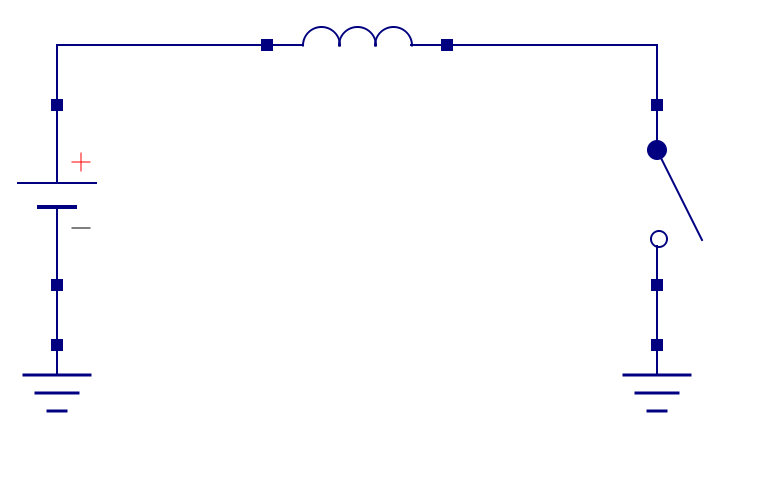
\includegraphics[width = 0.4\textwidth]{c-1.png}
\caption{Создание начального тока в катушке}
\end{figure}

\subsection*{Нагнетание напряжения на конденсаторе}

После создания в катушке некоторого тока его можно <<пустить>> его (размыканием ключа) в другом направлении. <<Отправим>> ток на конденсатор ёмкости $C = 10$ мкФ:\\

\begin{figure}[h!]
\centering
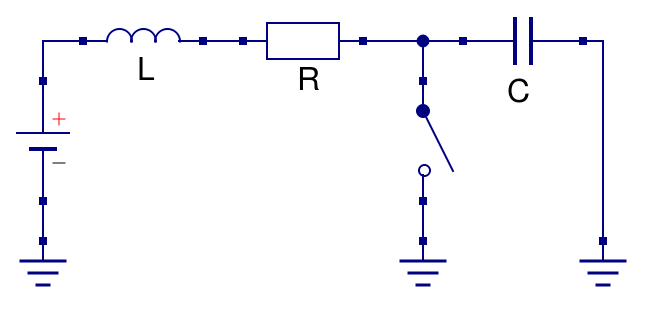
\includegraphics[width = 0.4\textwidth]{c-4.png}
\caption{Схема с подключенным конденсатором}
\end{figure}





\section*{Первые расчёты}
Сразу перейдём к практике. Здесь и далее воспользуемся источником DC напряжения с $U_0 = 10$ В.

Реальные катушки имеют конечное активное сопротивление (обыкновенное сопротивление постоянному току). Здесь и далее будем рассматривать катушку с $R = 1$ Ом и $L = 200$ мкГн (вполне типичные параметры для катушки с сердечником, подходящим для работы в режиме преобразования напряжения). Также разумно использовать обозначение для характерного времени установления тока в катушке $\tau = L/R$. Будем рассматривать \textbf{эквивалентную схему} с последовательно соединенными идеальной катушкой и резистором.\\

\begin{figure}[h!]
\centering
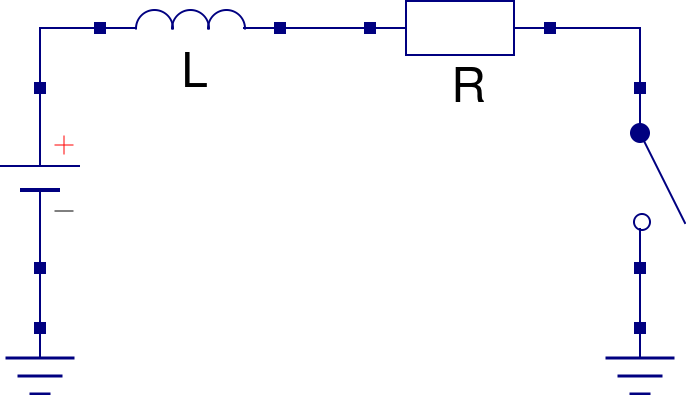
\includegraphics[width = 0.4\textwidth]{c-2.png}
\caption{Эквивалентная схема с активным сопротивлением катушки}
\end{figure}


Чтобы развить в катушке некоторый ток, придётся потерять часть энергии из-за потерь на резисторе, поэтому нет смысла держать ключ открытым слишком долгое время. Выясним, как эти потери зависят от времени.\\

Для создания преобразователя используем микросхему MAX1771, работающую на частоте $\nu = 300$ кГц. А значит, следует дальнейшие вычисления проводить для времен открытия ключа порядка $t_\text{пр} = 1/\nu$ (очевидно, время $t_\text{пр} \ll \tau$). Это позволит сильно упростить полученные уравнения.\\


\begin{enumerate}[resume]
\item Найдём зависимость тока, возбужденного в катушке, от  времени. Операторный коэффициент передачи
$$K(p) = \frac{R}{pL+R},$$
значит, ток в катушке
$$I(t) = U_R(t)/R \risingdotseq\frac{1}{R}\mathcal{L}(U(t)) = \frac{1}{p(p+R/L)} \risingdotseq \frac{U_0}{R} \left(1-e^{-t/\tau}\right) \simeq \frac{U_0}{R} \frac{t}{\tau}.$$

\item Подсчитаем также джоулевы потери на резисторе за это время (это, очевидно, необходимо для расчёта КПД преобразователя):
$$W_R(t) = \int_{0}^{t} I^{2}(t) R\ dt \simeq \frac{U_0^2}{R} \frac{t^3}{3\tau^2}.$$

\item После размыкания ключа процессы в цепи описываются обычным дифференциальным уравнением второго порядка для LRC-цепочки. Имеем
$$LC \ddot U +R \dot U + U = U_0,$$
где за $U$ обозначено напряжение на конденсаторе. Общее решение -- затухающие (апериодические колебания).

Приводим качественный график решения для начального напряжения на конденсаторе $U_C = U_0$:

\begin{figure}[H]
\centering
\begin{gnuplot}[terminal=epslatex]
set samples 10000
set xrange [0:10]
set yrange [9:11]
set ylabel "$U$, \\V"
set xlabel "$t$, \\ms"
set key off
set grid
set size 1.3,1.2
f(x) = 10*(0.1*sin(3*x)*exp(-x*0.3)+1)
plot f(x) lw 3 lc 6
\end{gnuplot}
\end{figure}

Видно, что после размыкания ключа на конденсаторе происходит скачок напряжения на конденсаторе до значений, больших $U_0$ (также, как это происходило в первой части задачи).
К сожалению, с приходом следующего периода достигнутый результат <<теряется>>, напряжение быстро падает до начального (см. график $U(t)$). Но если в схему добавить диод, пропускающий ток только в одном направлении, то ток не сможет течь в обратном направлении, и на конденсаторе останется максимальное напряжение:\\

\begin{figure}[H]
\centering
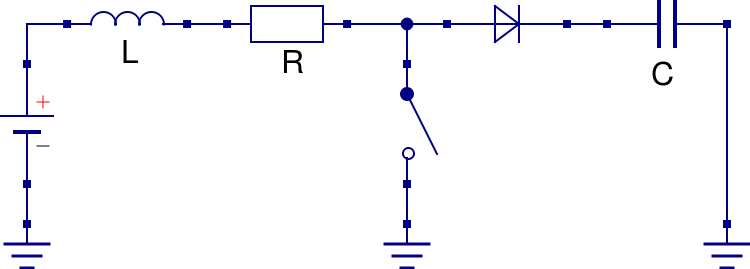
\includegraphics[width = 0.4\textwidth]{c-5.png}
\caption{Схема с добавленным диодом}
\end{figure}

\end{enumerate}

\section*{Большие напряжения}
\begin{enumerate}[resume]
\item Теперь будем предполагать начальное напряжение на конденсаторе достаточно большим, $U_C$ = 100 В. Это сильно упростит полученное дифференциальное уравнение, так как скачок напряжения $U_\text{ск} \ll U_C$ (проверим это). 

Найдём этот скачок напряжения. Сделаем замену $\varphi = U-U_0$, уравнение примет вид
$$\ddot \varphi + 2\gamma \dot \varphi + \omega_0^2 \varphi = 0,$$
где, как обычно, $\omega_0^2 = 1/LC$, $\gamma = R/2L$.

Примерный график в этом случае выглядит так:
\begin{figure}[H]
\centering
\begin{gnuplot}[terminal=epslatex]
set samples 10000
set xrange [0:10]
set yrange [-100:100]
set ylabel "$U$, \\V"
set xlabel "$t$, \\ms"
set key off
set grid
set size 1.3,1.2
f(x) = 100*cos(3*x-0.6)*exp(-x*0.3)
plot f(x) lw 3 lc 6
\end{gnuplot}
\end{figure}

При условии $\Delta t \ll T$ в разложении решения в ряд Тейлора в точке максимума $t_0$ можно ограничиться производной второго порядка:
$$\varphi(t_0+\Delta t) \simeq \varphi(t_0) + \cancelto{\scriptstyle 0}{\dot \varphi(t_0) \Delta t}~~+ \ddot \varphi(t_0) \frac{\Delta t^2}{2}.$$
Учитывая, что в максимуме $\ddot \varphi =  - \omega_0^2 \varphi(t_0)$, и $\varphi(t_0) = \varphi(0)+U_\text{ск}$, а также, что $I = C \dot \varphi$ и $\dot \varphi (0) \simeq - \ddot \varphi \Delta t$, имеем
$$\Delta t = \frac{LI}{\varphi(0)}, \quad U_\text{ск} = I^2 \frac{L}{2C} \frac{1}{\varphi(0)},$$
причём из условия $\Delta t  \ll T$ следует 
$$I \ll \sqrt{\frac{C}{L}} \varphi(0).$$

\item Проверим, что это соотношение выполнено даже для максимально возможного тока $I$ в катушке (время возбуждения тока в катушке равно $t_\text{пр}$):
$$I_{\max} = \frac{U_0}{R} \frac{t_\text{пр}}{\tau} = 0,165~\A, \quad \sqrt{\frac{C}{L}} \varphi(0) = 20,1~\A$$ 

\end{enumerate}

\section*{Реальный преобразователь}

Теперь, чтобы повышать напряжение и дальше, нужно периодически замыкать и размыкать ключ. Тогда напряжение на конденсаторе будет скачками расти (хотя, очевидно, скачки будут тем слабее, чем больше напряжение конденсатора). Реально преобразователь работает следующим образом. Клеммы конденсатора есть выход схемы, к выходу подключают нагрузку, через которую течет ток, разряжающий конденсатор. А специализированная микросхема в это же время с высокой частотой открывает и закрывает ключ, подкачивая в конденсатор энергию и компенсируя потерю напряжения.\\

\subsection*{Расчёт работы преобразователя}

Пусть на конденсаторе установилось стационарное напряжение $U_C = 100$ В. Предполагаем, что в нагрузку течет такой ток, что он полностью компенсирует рост напряжения в результате работы схемы, описанной выше, т.е. напряжение на конденсторе неизменно.

Считаем, что ключ замыкается на время $t_L$, размыкается на $t_\text{пр} - t_L$ (то есть имеем меандр со скважностью $s = t_L/t_\text{пр}$:

\begin{figure}[H]
\centering
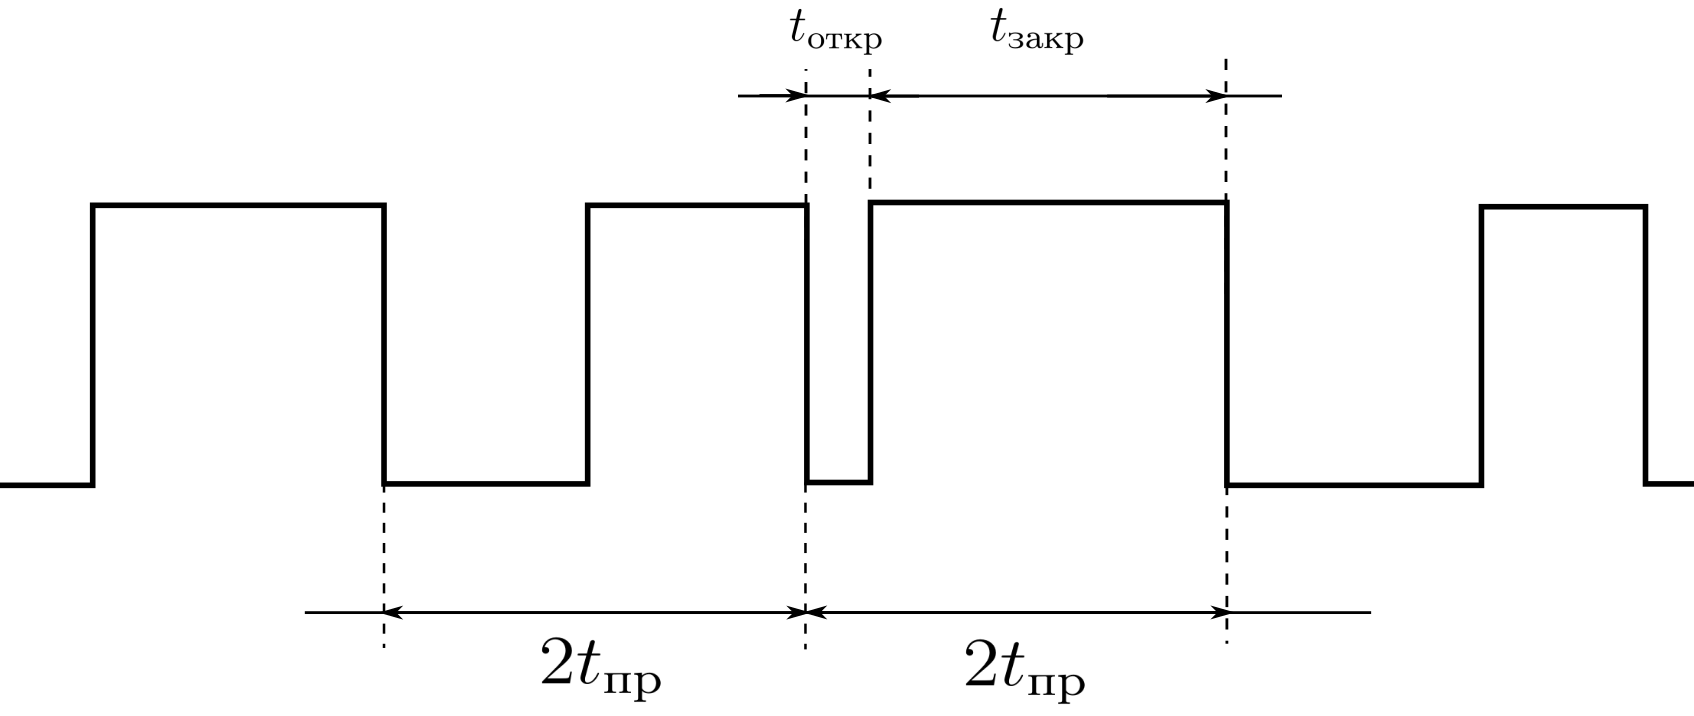
\includegraphics[width = 0.9\textwidth]{c-6.png}
\caption{График меандра переменной скважности}
\end{figure}

\begin{enumerate}[resume]

\item Считаем, что скважность сигнала не слишком велика, так что $t_0 < t_\text{пр} - t_L$ (это верно при скважности, меньшей, чем 
$$ s_{\max} = \frac{1}{1+U_0/\varphi(0)} = 0,9,$$
т.\,е. скважность лежит в пределах $[0; 0,9]$. 



\end{enumerate}

\section*{Стабилизация напряжения}

Реальный преобразователь должен подстраиваться под значение тока в нагрузке, стабилизируя напряжение на выходе (в противном случае либо мощности будет не хватать, и заряд с конденсатора быстро стравится в нагрузку, либо преобразователь будет нагнетать слишком большое напряжение на выходе). Для этого при уменьшении тока нагрузки уменьшается скважность меандра, управляющего ключом.



Тогда за период работы преобразователя в катушке возбуждается меньший ток, конденсатору передается меньшая энергия. В пределе, когда нагрузка отключена, а утечки конденсатора пренебрежимо малы, скважность сигнала стремится к 100\% (ключ всегда закрыт, ток не течет).\\


\begin{enumerate}[resume]
\item Найдём зависимость скважности сигнала меандра от тока нагрузки:
$$U_\text{ск} = \frac{\Delta q}{C}=  \frac{\left< I \right> t_\text{пр}}{C},$$
поэтому окончательно получаем
$$\left< I \right> = \frac{CU_\text{ск}}{t_\text{пр}} = \frac{s^2}{\nu} \frac{U_0}{U_\text{вых}-U_0} \frac{U_0}{2L}.$$
Производя расчёты, получим 
$$I = s^2 \cdot 9,3~\m\A,$$
то есть максимальный ток, который может течь в нагрузке в рассмотренном режиме работы преобразователя
$$I_{\max} = 0,9^2 \cdot 9~\m\A = 7,5~\m\A.$$
\end{enumerate} 


\section*{Мощность и КПД преобразователя}
\begin{enumerate}[resume]
\item Зная выходной ток и напряжение, можем посчитать выходную мощность перобразователя:
$$W = \frac{s^2}{\nu} \frac{U_0 U_\text{вых}}{U_\text{вых}-U_0} \frac{U_0}{2L} \simeq \Big| U_0 \ll U_\text{вых} \Big| \simeq \frac{s^2}{\nu} \frac{U_0^2}{2L}.$$

Видно, что увеличение индуктивности катушки и/или частоты преобразования ведёт к уменьшению выходной мощности преобразователя. Однако повысить мощность, уменьшив эти величины, на практике затруднительно, потому что уменьшение и той, и другой ведёт к увеличению максимального тока, протекающего по катушке:
$$I_{\max} = \frac{U_0}{\nu L}.$$

Таким образом заключаем, <<чудес не бывает>>, т.\,е. при попытке увеличить мощность преобразователя мы наталкиваемся на непреодолимую физическую трудность в виде необходимости увеличивать максимальный ток катушки, что приводит к увеличению её размеров, и, как следствие, к увеличению размеров конечного устройства. Более совершенные схемы позволяют в какой-то степени обойти это ограничение, однако его общий характер сохраняется (так, блок питания ноутбука всегда значительно больше блока питания телефона). 
\end{enumerate}

\subsection*{КПД преобразователя}
\begin{enumerate}[resume]
\item Практически важным вопросом также является КПД такого преобразователя. Выходная мощность уже известна. Подсчитаем работу источника.
Работа по возбуждению тока в катушке:
$$A_1 = \int_0^t U_0 I ~ dt = \frac{U_0^2}{\nu^2} \frac{s^2}{2L}$$
Работа источника после размыкания ключа:
$$A_2 = U_0 \Delta q = U_0 C U_\text{ск} = \frac{U_0 \left< I \right>}{\nu} = \frac{s^2}{\nu^2} \frac{U_0^2}{U_\text{вых}-U_0} \frac{U_0}{L}$$

Полная мощность источника
$$W_\text{ист} = \frac{A_1+A_2}{t_\text{пр}} = \frac{U_0^2}{\nu} \frac{s^2}{2L} \left( 1+ \frac{2U_0}{U_\text{вых} - U_0} \right).$$
\item Окончательно получим для КПД системы
$$\eta = \frac{W}{W_\text{ист}} = \frac{1}{1+\tfrac{2U_0}{U_\text{вых}-U_0}} \cdot \frac{U\text{вых}}{U_\text{вых}-U_0} = \frac{1}{1+\tfrac{U_0}{U_\text{вых}}} \simeq \Big| U_0 \ll U_\text{вых} \Big| \simeq 1.$$

Мы получили примечательное соотношение, которое показывает, что КПД импульсного преобразователя сверху ограничен только единицей, и не падает (а, согласно нашей формуле, даже растёт) с ростом разницы напряжений. Этот вывод, конечно, не учитывает прочих потерь в схеме (см. экспериментальную часть), которые, вообще говоря, растут с ростом напряжения, а, значит, не может считаться вполне правильным. Но он показывает, что для КПД такой схема нет \textbf{принципиальных} ограничений сверху.
\end{enumerate}


\section*{Пару слов о существующих схемах}

\begin{figure}[H]
\centering
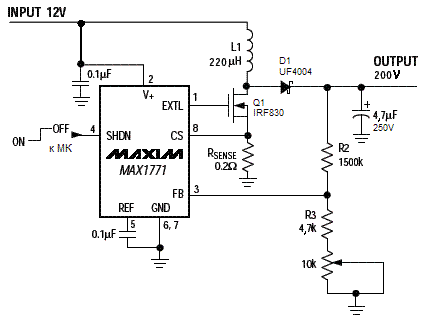
\includegraphics[width = 0.5\textwidth]{c-7.png}
\caption{Принципиальная схема преобразователя}
\end{figure}

И реальный вид:\\

\begin{figure}[H]
\centering   
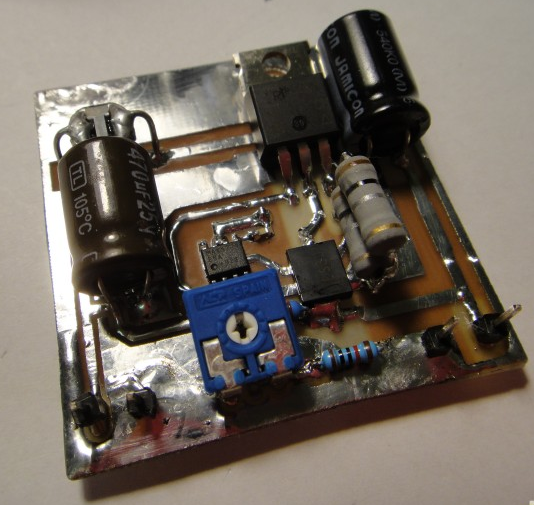
\includegraphics[width = 0.5\textwidth]{c-8.png}
\caption{Фото собранного перобразователя}
\end{figure}

\begin{enumerate}[resume]
\item В схеме кроме описанных в работе элементов есть два дополнительных: резистор $R_\text{SENSE}$, по напряжению на котором определяется и ограничивается максимальный ток в цепи, предохраняя преобразователь от короткого замыкания и перенагрузки), и резисторный делитель $R2-R3-10k$, с помощью которого микросхема и <<определяет>> напряжение на выходе преобразователя.


\end{enumerate}

\section*{Экспериментальная часть}
Для проверки теоретически полученных результатов измерим КПД преобразователя и снимем зависимость $I(s)$, подключая к выходу преобразователя потенциометр и варьируя его сопротивление.

\subsection*{Измерение КПД}
\begin{table}[H]
\centering
\begin{tabular}{|l|l|l|l|l|}
\hline
$I_\text{вх},~\m\A$ & $U_\text{вх},~\V$ & $I_\text{вых},~\m\A$ & $U_\text{вых},~\V$ & $\eta,~\%$ \\ \hline
22,8          & 12,0          & 2              & 182                  & 75        \\ \hline
35,0          & 12,0          & 3              & 182                  & 77        \\ \hline
57,6          & 12,0          & 5              & 182                  & 76        \\ \hline
72,8          & 12,0          & 6              & 182                  & 80        \\ \hline
98,2          & 12,0          & 8              & 182                  & 81        \\ \hline
124,4         & 12,0          & 10             & 182                  & 82        \\ \hline
195,9         & 12,0          & 15             & 182                  & 86        \\ \hline
\end{tabular}
\caption{измерение КПД при разных нагрузках}
\end{table}

Заметно, что в силу особенностей работы схемы проявляется зависимость КПД от тока в нагрузке. Выявить явный вид этой зависимости не удалось, но теоретическая оценка на среднее значение КПД даёт приблизительно верный результат (разумеется, завышенный, ведь мы не учитывали ни питание микроконтроллера, ни дополнительные потери в катушке, ни утечки конденсатора, ни даже потери в ключевом транзисторе):
$$\left< \eta \right> \approx (80 \pm 6)~\%,$$
$$\eta_\text{теор} = 93~\%.$$
\pagebreak
\subsection*{Измерение зависимости тока от скважности сигнала}
Чтобы убедиться в справедливости наших изысканий, снимем упомянутую зависимость:

\begin{figure}[H]
\centering
\begin{gnuplot}[terminal=epslatex]
set samples 10000
set xrange [0:1]
set yrange [0:18]
set ylabel "$I,$ \\m\\A"
set xlabel "$s$"
set key off
set grid
set size 1.2,1.1

f(x) = 17*(x**2)/(0.8**2)
plot "data1.dat" using 2:1 ps 3 pt 7 lc 6, f(x) lc 6 lw 5
\end{gnuplot}
\caption{Аппроксимация полученной зависимости параболой}
\end{figure}

Лианеризованный график:

\begin{figure}[H]
\centering
\begin{gnuplot}[terminal=epslatex]
set samples 10000
set xrange [0:0.8]
set yrange [0:18]
set ylabel "$I,$ \\m\\A"
set xlabel "$s^2$"
set key off
set grid
set size 1.2,1.1

f(x) = a*x
fit f(x) "data2.dat" using 2:1 via a
plot "data2.dat" using 2:1 ps 3 pt 7 lc 6, f(x) lc 6 lw 5
\end{gnuplot}
\caption{Лианеризованная зависимость}
\end{figure}

\pagebreak
\section*{Выводы}
\begin{enumerate}
\item Успешно разработана схема преобразователя
\item Схема реализована на монтажной плате и протестирована
\item Изучен принцип работы схемы
\item Из чисто физических соображений были получены практически важные зависимости, имеющие значение при разработке преобразователей
\item Упомянутые зависимости были качественно проверены экспериментом
\end{enumerate}

\end{document}